% Hand-written against the original team class, with the same content as
% golden.qmd. Compiling this file produces reference.pdf, the page images the
% Galley output must match.
\documentclass{whitepaper}
\usepackage[round,authoryear]{natbib}
\bibliographystyle{plainnat}

\title{Liquidity Stress Testing Framework}
\subtitle{Golden fidelity document}
\author{Risk Analytics Team \and Treasury Modelling}
\date{October 2026}
\docid{WP-TEST-001}
\classification{Confidential}
\docversion{0.9}

\begin{document}
\maketitle

\begin{abstract}
This document exercises every feature of the team template so that the
Galley output can be compared, page by page, with the same content typeset
directly through the original class.
\end{abstract}

\section{Introduction}\label{sec-intro}

Liquidity stress testing follows the supervisory framework
\citep{bcbs2013}. The classic account of bank runs is
\citet{diamond1983}. Text can carry \emph{emphasis}, \textbf{strong
emphasis} and \texttt{inline code}, and a footnote.\footnote{The survival
horizon is 30 calendar days, costing \$1.2m a year to monitor.}

\subsection{Scope}

The framework covers three things:

\begin{itemize}
\item retail and wholesale deposits;
\item committed credit and liquidity facilities;
\item collateral calls on derivatives.
\end{itemize}

It is applied in two steps:

\begin{enumerate}
\item Project contractual and behavioural cash flows.
\item Compare cumulative net outflows with the liquidity buffer.
\end{enumerate}

\subsubsection{Scenario design}

Scenarios combine market-wide and firm-specific shocks.

\paragraph{Idiosyncratic stress}

A two-notch downgrade triggers wholesale funding run-off of 40\%.

\paragraph{Market stress}

Haircuts on level 2 assets widen by 15 percentage points.

\begin{keyfinding}
The 30-day survival horizon is met in every scenario, with a minimum
buffer of 112\% of net outflows.
\end{keyfinding}

\begin{recommendation}[Next step]
Recalibrate deposit outflow rates every quarter.
\end{recommendation}

\section{Results}\label{sec-results}

Figure~\ref{fig-survival} shows the survival curve and
Table~\ref{tbl-outflows} lists the outflow assumptions discussed in
Section~\ref{sec-intro}.

\begin{figure}
\centering
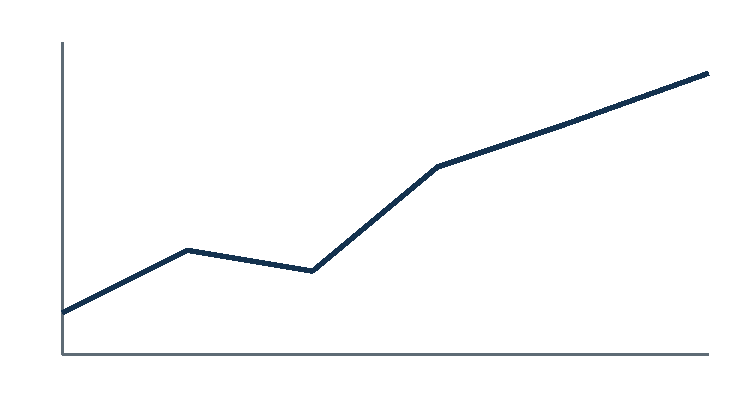
\includegraphics[width=0.7\linewidth]{survival-curve.pdf}
\caption{Cumulative liquidity buffer over the stress horizon}\label{fig-survival}
\end{figure}

{\small
\begin{longtable}{@{}lrr@{}}
\caption{Outflow assumptions by deposit category}\label{tbl-outflows}\\
\toprule
Category & Outflow rate & Balance (\$m) \\
\midrule
\endhead
\bottomrule
\endlastfoot
Stable retail & 5\% & 12,400 \\
Less stable retail & 10\% & 6,150 \\
Operational & 25\% & 3,980 \\
Non-operational & 40\% & 2,275 \\
\end{longtable}
}

The liquidity coverage ratio is
\(\mathit{LCR} = \mathit{HQLA} / \mathit{NCO} \ge 100\%\).

\bibliography{references}
\end{document}
